\documentclass{article}

% content/resources/templates/preamble.tex
\usepackage[margin=0.6in]{geometry}
\author{Milav Dabgar}
\usepackage{amsmath,amssymb,amsthm}
\usepackage{booktabs}
\usepackage{multirow}
\usepackage{xcolor}
\usepackage{tcolorbox}
\tcbuselibrary{breakable,skins}
\usepackage[colorlinks=true,linkcolor=blue]{hyperref}
\usepackage{titlesec}
\usepackage{enumitem}
\usepackage{tikz}
\usepackage{pgfplots}
\usepackage{circuitikz}
\usepackage[version=4]{mhchem}
\usepackage{longtable}
\usepackage{array}
\usepackage{float}
\usepackage{caption}
\usepackage{listings}

\lstset{
  basicstyle=\small\ttfamily,
  breaklines=true,
  breakatwhitespace=false,
  postbreak=\mbox{\textcolor{red}{$\hookrightarrow$}\space},
  float=false,
  numbers=left,
  numberstyle=\tiny\color{gray},
  numbersep=10pt,
  xleftmargin=2em,
  keywordstyle=\color{blue},
  commentstyle=\color{green!60!black},
  stringstyle=\color{purple},
  backgroundcolor=\color{gray!5},
  showstringspaces=false,
  tabsize=2,
  captionpos=b,
  keepspaces=true,
  columns=flexible
}

\pgfplotsset{compat=1.18}
\usetikzlibrary{shapes,arrows,positioning,calc,patterns,decorations.pathmorphing,decorations.markings,arrows.meta}

% Color scheme
\definecolor{headcolor}{RGB}{0,102,204}
\definecolor{keycolor}{RGB}{220,20,60}
\definecolor{solutioncolor}{RGB}{34,139,34}
\definecolor{mnemoniccolor}{RGB}{148,0,211}
\definecolor{codecolor}{RGB}{0,0,100}

% Spacing
\setlength{\parskip}{3pt}
\setlist[itemize]{nosep}
\setlist[enumerate]{nosep}

% Title formatting
\titleformat{\section}{\Large\bfseries\color{headcolor}}{\thesection}{1em}{}
\titleformat{\subsection}{\large\bfseries\color{headcolor}}{\thesubsection}{1em}{}

% Pandoc tightlist compatibility
\providecommand{\tightlist}{%
  \setlength{\itemsep}{0pt}\setlength{\parskip}{0pt}}

% Pandoc longtable compatibility
\newcounter{none}
\def\thenone{}


% content/resources/templates/english-boxes.tex

% Custom environments
\newtcolorbox{solutionbox}{
 breakable,
 enhanced,
 colback=solutioncolor!5!white,
 colframe=solutioncolor!75!black,
 fonttitle=\bfseries,
 title=Solution
}

\newtcolorbox{solutionboxnobreak}{
 colback=solutioncolor!5!white,
 colframe=solutioncolor!75!black,
 fonttitle=\bfseries,
 title=Solution
}

\newtcolorbox{keyformula}{
 breakable,
 enhanced,
 colback=keycolor!5!white,
 colframe=keycolor!75!black,
 fonttitle=\bfseries,
 title=Key Formula
}

\newtcolorbox{mnemonicboxenv}{
 breakable,
 enhanced,
 colback=mnemoniccolor!5!white,
 colframe=mnemoniccolor!75!black,
 fonttitle=\bfseries,
 title=Mnemonic
}

\newcommand{\mnemonicbox}[1]{%
  \begin{mnemonicboxenv}
    #1
  \end{mnemonicboxenv}
}


% Custom commands for GTU solutions
% This file defines semantic commands for consistent formatting

% Question command with automatic formatting
\newcommand{\question}[2]{%
  \section*{Question #1}%
  \textbf{#2}%
}

% OR question variant
\newcommand{\questionor}[2]{%
  \section*{Question #1 OR}%
  \textbf{#2}%
}

% Proper table environment with caption
\newenvironment{answertable}[1]{%
  \begin{table}[htbp]
  \centering
  \caption{#1}
}{%
  \end{table}
}

% Proper figure environment for diagrams
\newenvironment{answerdiagram}[1]{%
  \begin{figure}[htbp]
  \centering
  \caption{#1}
}{%
  \end{figure}
}

% Semantic markup for key terms
\newcommand{\keyword}[1]{\textbf{#1}}
\newcommand{\code}[1]{\texttt{#1}}
\newcommand{\classname}[1]{\texttt{#1}}
\newcommand{\methodname}[1]{\texttt{#1}}

% Proper quotation marks
\newcommand{\mnemonic}[1]{``#1''}


\title{Electronic Measurements and Instruments (4331102) - Winter 2022 Solution}
\date{February 27, 2023}

\begin{document}
\maketitle

\questionmarks{1(a)}{3}{Draw and explain working of Basic Q-Meter.}

\begin{solutionbox}
\textbf{Q-meter} is an instrument used to measure the quality factor (Q) of an inductor or capacitor.

\textbf{Block Diagram}:
\begin{center}
\begin{tikzpicture}[node distance=1.5cm, auto]
    \node [gtu block] (Osc) {Oscillator};
    \node [gtu block, right=of Osc] (Amp) {Amplifier};
    \node [gtu block, right=of Amp] (Res) {Resonance Circuit};
    \node [gtu block, right=of Res] (Volt) {Voltage Ind.};
    \node [gtu block, below=of Res] (DUT) {DUT};
    
    \draw [gtu arrow] (Osc) -- (Amp);
    \draw [gtu arrow] (Amp) -- (Res);
    \draw [gtu arrow] (Res) -- (Volt);
    \draw [gtu arrow] (Res) -- (DUT);
    \draw [gtu arrow] (DUT) -- (Res);
\end{tikzpicture}
\captionof{figure}{Basic Q-Meter Block Diagram}
\end{center}

\textbf{Functions}:
\begin{itemize}
    \item \keyword{Oscillator}: Generates variable frequency signal.
    \item \keyword{Amplifier}: Amplifies the signal to required level.
    \item \keyword{Resonance Circuit}: Contains the component under test and tuning elements.
    \item \keyword{Voltage Indicator}: Measures the voltage across the component (V) relative to input (E).
\end{itemize}
\end{solutionbox}

\begin{mnemonicbox}
\mnemonic{OARV - Oscillate, Amplify, Resonate, View}
\end{mnemonicbox}

\questionmarks{1(b)}{4}{Explain Spectrum Analyzer in brief.}

\begin{solutionbox}
A \textbf{Spectrum Analyzer} measures the magnitude of an input signal versus frequency within the full frequency range of the instrument.

\textbf{Block Diagram}:
\begin{center}
\begin{tikzpicture}[node distance=1.5cm, auto]
    \node [gtu block] (Mix) {Mixer};
    \node [gtu block, left=of Mix] (In) {Input};
    \node [gtu block, below=of Mix] (LO) {Local Osc.};
    \node [gtu block, right=of Mix] (IF) {IF Filter};
    \node [gtu block, right=of IF] (Det) {Detector};
    \node [gtu block, right=of Det] (Disp) {Display};
    
    \draw [gtu arrow] (In) -- (Mix);
    \draw [gtu arrow] (LO) -- (Mix);
    \draw [gtu arrow] (Mix) -- (IF);
    \draw [gtu arrow] (IF) -- (Det);
    \draw [gtu arrow] (Det) -- (Disp);
\end{tikzpicture}
\captionof{figure}{Spectrum Analyzer Block Diagram}
\end{center}

\textbf{Key Aspects}:
\begin{itemize}
    \item \keyword{Input Signal Processing}: Signals enter through attenuator and filters.
    \item \keyword{Frequency Domain Conversion}: Converts time domain to frequency domain.
    \item \keyword{Display System}: Shows amplitude vs. frequency plot.
    \item \keyword{Applications}: Signal analysis, distortion measurement, EMI testing.
\end{itemize}
\end{solutionbox}

\begin{mnemonicbox}
\mnemonic{SAME-FD: Signal Analysis Measures Everything in Frequency Domain}
\end{mnemonicbox}

\questionmarks{1(c)}{7}{Explain Wheatstone bridge with circuit diagram. List its advantages and disadvantages.}

\begin{solutionbox}
\textbf{Wheatstone bridge} is a circuit used to measure unknown resistance with high accuracy.

\textbf{Circuit Diagram}:
\begin{center}
\begin{circuitikz}[american, scale=0.8]
    \draw (0,3) node[left] {A} to[R, l=$R_1$] (3,5) node[above] {B} to[R, l=$R_3$] (6,3) node[right] {C};
    \draw (6,3) to[R, l=$R_x$] (3,1) node[below] {D} to[R, l=$R_2$] (0,3);
    \draw (3,5) to[rmeter, t=G] (3,1);
    \draw (0,3) to[short] (-1,3) to[battery1, l=$V$] (-1,1) to[short] (3,1); % Corrected connection
    % Re-drawing source connection better
    \draw (0,3) -- (-0.5,3) -- (-0.5, 0.5) to[battery1] (6.5, 0.5) -- (6.5, 3) -- (6,3);
\end{circuitikz}
\captionof{figure}{Wheatstone Bridge}
\end{center}

Where:
\begin{itemize}
    \item $R_1, R_2, R_3$ are known resistances.
    \item $R_x$ is unknown resistance.
    \item $G$ is galvanometer.
\end{itemize}

\textbf{Working Principle}:
\begin{itemize}
    \item Bridge is balanced when potential at B equals potential at D and no current flows through G.
    \item \keyword{Balance Condition}: $\frac{R_1}{R_2} = \frac{R_3}{R_x}$
    \item \keyword{Unknown Resistance}: $R_x = R_3 (\frac{R_2}{R_1})$
\end{itemize}

\begin{center}
\captionof{table}{Advantages and Disadvantages}
\begin{tabulary}{\linewidth}{|L|L|}
\hline
\textbf{Advantages} & \textbf{Disadvantages} \\ \hline
High accuracy & Limited range \\ \hline
Good sensitivity & Temperature effects \\ \hline
Null type measurement & Requires balance adjustment \\ \hline
No need for calibrated meter & Not suitable for very low/high resistances \\ \hline
\end{tabulary}
\end{center}
\end{solutionbox}

\begin{mnemonicbox}
\mnemonic{BARN - Balance Achieved when Ratios are Null}
\end{mnemonicbox}

\questionmarks{1(c) OR}{7}{Define Instrument and explain its characteristics.}

\begin{solutionbox}
An \textbf{instrument} is a device used for measuring, displaying or recording physical quantities.

\textbf{Instrument Block Diagram}:
\begin{center}
\begin{tikzpicture}[node distance=1.5cm, auto]
    \node [gtu block] (Inst) {Instrument};
    \node [coordinate, left=of Inst] (In) {};
    \node [coordinate, right=of Inst] (Out) {};
    \node [gtu block, above=of Inst] (Env) {Environmental};
    \node [gtu block, below=of Inst] (Err) {Errors};
    
    \draw [gtu arrow] (In) -- node[above]{Input} (Inst);
    \draw [gtu arrow] (Inst) -- node[above]{Reading} (Out);
    \draw [gtu arrow] (Env) -- (Inst);
    \draw [gtu arrow] (Err) -- (Inst);
\end{tikzpicture}
\captionof{figure}{General Instrument System}
\end{center}

\begin{center}
\captionof{table}{Instrument Characteristics}
\begin{tabulary}{\linewidth}{|L|L|}
\hline
\textbf{Characteristic} & \textbf{Description} \\ \hline
\keyword{Accuracy} & Closeness of measurement to true value \\ \hline
\keyword{Precision} & Repeatability of measurements \\ \hline
\keyword{Resolution} & Smallest change that can be detected \\ \hline
\keyword{Sensitivity} & Ratio of output signal to input signal change \\ \hline
\keyword{Linearity} & Proportional relationship between input and output \\ \hline
\keyword{Range} & Minimum to maximum measurable values \\ \hline
\keyword{Response time} & Time required to show true reading \\ \hline
\end{tabulary}
\end{center}

\textbf{Types}:
\begin{itemize}
    \item \textbf{Static Characteristics}: Properties that don't vary with time.
    \item \textbf{Dynamic Characteristics}: Properties that vary with time.
\end{itemize}
\end{solutionbox}

\begin{mnemonicbox}
\mnemonic{APRS-LRR: Accuracy and Precision, Resolution and Sensitivity, Linearity, Range, Response time}
\end{mnemonicbox}

\questionmarks{2(a)}{3}{Draw the construction diagram of Energy meter.}

\begin{solutionbox}
\textbf{Energy meter} measures electrical energy consumption in kilowatt-hours (kWh).

\textbf{Diagram}:
\begin{center}
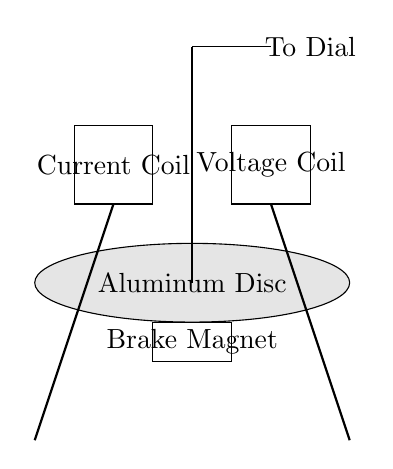
\begin{tikzpicture}
    % Disc
    \draw [fill=gray!20] (0,0) ellipse (2 and 0.5);
    \node at (0,0) {Aluminum Disc};
    \draw [thick] (0,0) -- (0,3); % Spindle
    \draw (0,3) -- (1,3); \node at (1.5,3) {To Dial};
    
    % Magnets/Coils
    \draw (-1.5, 1) rectangle (-0.5, 2); \node at (-1, 1.5) {Current Coil};
    \draw (0.5, 1) rectangle (1.5, 2); \node at (1, 1.5) {Voltage Coil};
    \draw (-0.5, -1) rectangle (0.5, -0.5); \node at (0, -0.75) {Brake Magnet};
    
    % Connections
    \draw [thick] (-2, -2) -- (-1, 1);
    \draw [thick] (2, -2) -- (1, 1);
\end{tikzpicture}
\captionof{figure}{Induction Type Energy Meter}
\end{center}

\textbf{Components}:
\begin{itemize}
    \item \keyword{Rotating Aluminum Disc}: Moves proportional to power.
    \item \keyword{Current Coil}: Creates flux proportional to current.
    \item \keyword{Voltage Coil}: Creates flux proportional to voltage.
    \item \keyword{Permanent Magnet}: Provides braking torque.
\end{itemize}
\end{solutionbox}

\begin{mnemonicbox}
\mnemonic{DVCP: Disc Velocity measures Consumed Power}
\end{mnemonicbox}

\questionmarks{2(b)}{4}{Explain working of PMMC in short.}

\begin{solutionbox}
\textbf{PMMC (Permanent Magnet Moving Coil)} is a basic mechanism used in various DC meters.

\textbf{Construction Diagram}:
\begin{center}
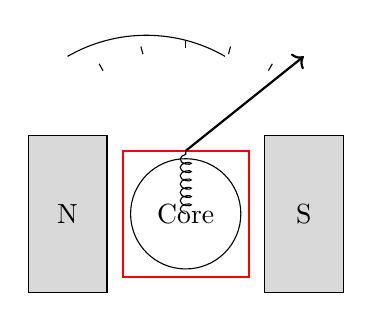
\begin{tikzpicture}
    % Magnets
    \draw [fill=gray!30] (-2, -1) rectangle (-1, 1); \node at (-1.5, 0) {N};
    \draw [fill=gray!30] (1, -1) rectangle (2, 1); \node at (1.5, 0) {S};
    % Core
    \draw (0,0) circle (0.7); \node at (0,0) {Core};
    % Coil
    \draw [thick, color=red] (-0.8, -0.8) rectangle (0.8, 0.8);
    % Pointer
    \draw [thick, ->] (0, 0.8) -- (1.5, 2);
    % Scale
    \draw (0.5, 2) arc (60:120:2);
    \foreach \x in {60, 75, 90, 105, 120} \draw (\x:2.1) -- (\x:2.2);
    % Spring
    \draw [decorate, decoration={coil, segment length=3pt, amplitude=2pt}] (0,0) -- (0, 0.8);
\end{tikzpicture}
\captionof{figure}{PMMC Construction}
\end{center}

\begin{center}
\captionof{table}{Key Components}
\begin{tabulary}{\linewidth}{|L|L|}
\hline
\textbf{Component} & \textbf{Function} \\ \hline
Permanent Magnet & Creates strong magnetic field \\ \hline
Moving Coil & Carries current to be measured \\ \hline
Spring & Provides controlling torque \\ \hline
Pointer & Indicates reading on scale \\ \hline
\end{tabulary}
\end{center}

\textbf{Working}: When current flows through the coil placed in a magnetic field, a force is exerted on it, producing a deflecting torque $T_d \propto I$.
\end{solutionbox}

\begin{mnemonicbox}
\mnemonic{CODA: Current through cOil causes Deflection by Attraction}
\end{mnemonicbox}

\questionmarks{2(c)}{7}{1- A moving coil ammeter reading up to 1 ampere has a resistance of 0.02 ohm. How this instrument could be adopted to read current up to 100 amperes? 2- A moving coil voltmeter reading up to 20 mV has a resistance of 2 ohms. How this instrument can be adopted to read voltage up to 300 volts?}

\begin{solutionbox}
\textbf{Part 1: Ammeter Range Extension}

To extend ammeter range, a \keyword{Shunt Resistance ($R_sh$)} is connected in parallel.

\textbf{Diagram}:
\begin{center}
\begin{circuitikz}[american]
    \draw (0,2) to[short, i=$I$] (1,2) -- (4,2);
    \draw (2,2) to[R, l=$R_{sh}$] (2,0);
    \draw (3,2) to[rmeter, l=$R_m$, t=$A$] (3,0);
    \draw (1,0) -- (4,0);
\end{circuitikz}
\captionof{figure}{Ammeter with Shunt}
\end{center}

Given: $I_m = 1A$, $R_m = 0.02\Omega$, $I = 100A$.
Formula: $R_{sh} = \frac{R_m \cdot I_m}{I - I_m}$
Calculation:
$$ R_{sh} = \frac{0.02 \times 1}{100 - 1} = \frac{0.02}{99} \approx 0.000202\Omega $$

\textbf{Part 2: Voltmeter Range Extension}

To extend voltmeter range, a \keyword{Series Multiplier Resistance ($R_s$)} is connected in series.

\textbf{Diagram}:
\begin{center}
\begin{circuitikz}[american]
    \draw (0,0) to[R, l=$R_s$] (2,0) to[rmeter, l=$R_m$, t=$V$] (4,0);
    \draw (0,0) to[open, v=$V$] (4,0);
\end{circuitikz}
\captionof{figure}{Voltmeter with Multiplier}
\end{center}

Given: $V_m = 20mV = 0.02V$, $R_m = 2\Omega$, $V = 300V$.
Formula: $R_s = R_m (\frac{V}{V_m} - 1)$
Calculation:
$$ R_s = 2 \times (\frac{300}{0.02} - 1) = 2 \times (15000 - 1) = 2 \times 14999 = 29,998\Omega $$
\end{solutionbox}

\begin{mnemonicbox}
\mnemonic{SHIP: Shunt Has Inverse Proportion for current; Series for voltage}
\end{mnemonicbox}

\questionmarks{2(a) OR}{3}{Explain working of electronic multimeter.}

\begin{solutionbox}
\textbf{Electronic Multimeter} measures voltage, current, and resistance using active electronic components.

\textbf{Block Diagram}:
\begin{center}
\begin{tikzpicture}[node distance=1.5cm, auto]
    \node [gtu block] (Range) {Range Select};
    \node [gtu block, left=of Range] (Input) {Input};
    \node [gtu block, right=of Range] (Cond) {Signal Cond.};
    \node [gtu block, right=of Cond] (ADC) {ADC};
    \node [gtu block, right=of ADC] (Disp) {Display};
    
    \draw [gtu arrow] (Input) -- (Range);
    \draw [gtu arrow] (Range) -- (Cond);
    \draw [gtu arrow] (Cond) -- (ADC);
    \draw [gtu arrow] (ADC) -- (Disp);
\end{tikzpicture}
\captionof{figure}{Electronic Multimeter Block Diagram}
\end{center}

\textbf{Working}:
\begin{itemize}
    \item \keyword{Range Selection}: Attenuator/Amplifier network selects range.
    \item \keyword{Signal Conditioning}: Converts AC to DC, Current to Voltage, Resistance to Voltage.
    \item \keyword{ADC}: Analog to Digital Converter digitizes the signal.
    \item \keyword{Display}: LCD/LED shows the numeric value.
\end{itemize}
\end{solutionbox}

\begin{mnemonicbox}
\mnemonic{RSAD: Range Select, Amplify, Digitize}
\end{mnemonicbox}

\questionmarks{2(b) OR}{4}{Explain working of Moving Iron type instruments.}

\begin{solutionbox}
\textbf{Moving Iron instruments} utilize the magnetic force between a fixed coil and a moving iron piece.

\textbf{Working Principle}:
\begin{itemize}
    \item Current flows through a fixed coil, creating a magnetic field.
    \item Iron piece placed in the field gets magnetized.
    \item \keyword{Attraction Type}: Iron bar attracted into the coil.
    \item \keyword{Repulsion Type}: Two iron vanes magnetized with same polarity repel each other.
\end{itemize}

\textbf{Diagram (Repulsion Type)}:
\begin{center}
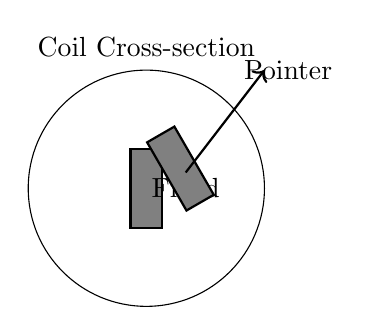
\begin{tikzpicture}
    \draw (0,0) circle (1.5);
    \node at (0,1.8) {Coil Cross-section};
    
    % Fixed Vane
    \draw [thick, fill=gray] (-0.2, -0.5) rectangle (0.2, 0.5); \node at (0.5, 0) {Fixed};
    % Moving Vane
    \draw [thick, fill=gray, rotate=30] (0.3, -0.5) rectangle (0.7, 0.5); 
    \draw [thick, ->] (0.5, 0.2) -- (1.5, 1.5); \node at (1.8, 1.5) {Pointer};
    
\end{tikzpicture}
\captionof{figure}{Moving Iron Mechanism}
\end{center}

\textbf{Features}: Non-linear scale, Used for AC \& DC, Robust.
\end{solutionbox}

\begin{mnemonicbox}
\mnemonic{CADS: Current Activates, Deflection Shows}
\end{mnemonicbox}

\questionmarks{2(c) OR}{7}{Draw the block diagram of Ramp type DVM. Illustrate process of obtaining Multirange DC voltmeter with circuit diagram.}

\begin{solutionbox}
\textbf{Ramp Type DVM} converts voltage to time ($V \propto t$).

\textbf{Block Diagram}:
\begin{center}
\begin{tikzpicture}[node distance=1.5cm, auto]
    \node [gtu block] (Comp) {Comparator};
    \node [gtu block, left=of Comp] (In) {Input};
    \node [gtu block, below=of Comp] (Ramp) {Ramp Gen};
    \node [gtu block, right=of Comp] (Gate) {Gate};
    \node [gtu block, right=of Gate] (Count) {Counter};
    \node [gtu block, right=of Count] (Disp) {Display};
    \node [gtu block, below=of Gate] (Osc) {Oscillator};
    
    \draw [gtu arrow] (In) -- (Comp);
    \draw [gtu arrow] (Ramp) -- (Comp);
    \draw [gtu arrow] (Comp) -- (Gate);
    \draw [gtu arrow] (Osc) -- (Gate);
    \draw [gtu arrow] (Gate) -- (Count);
    \draw [gtu arrow] (Count) -- (Disp);
\end{tikzpicture}
\captionof{figure}{Ramp Type DVM}
\end{center}

\textbf{Multirange DC Voltmeter Circuit}:
To measure different voltage ranges, a voltage divider network is used.

\begin{center}
\begin{circuitikz}[american]
    \draw (0,4) node[left]{$V_{in}$} to[short, o-] (1,4) -- (1,0); 
    \draw (1,4) to[R, l=$R_1$] (3,4);
    \draw (1,3) to[R, l=$R_2$] (3,3);
    \draw (1,2) to[R, l=$R_3$] (3,2);
    
    \draw (3,4) node[right]{Range 1};
    \draw (3,3) node[right]{Range 2};
    \draw (3,2) node[right]{Range 3};
    
    \draw (4,4) to[short] (4,2);
    \draw (4,3) to[short] (5,3) to[short] (5,1) -- (6,1);
    \node[draw] at (6.5,1) {DVM};
    \draw (0,0) node[left]{COM} to[short, o-] (6,0) -- (6,0.5);
    
    \node at (3.5, 5) {Selector Switch};
\end{circuitikz}
\captionof{figure}{Multirange Attenuator}
\end{center}
\end{solutionbox}

\begin{mnemonicbox}
\mnemonic{CRCD: Compare Ramp, Count Duration}
\end{mnemonicbox}

\questionmarks{3(a)}{3}{Describe features of Digital storage oscilloscope (DSO).}

\begin{solutionbox}
\textbf{Features of DSO}:
\begin{itemize}
    \item \keyword{Digital Storage}: Stores waveforms in memory for infinite time.
    \item \keyword{Pre-trigger Viewing}: Can see events before the trigger point.
    \item \keyword{Automatic Measurements}: Calculates Vpp, Vrms, Freq automatically.
    \item \keyword{PC Connectivity}: USB/LAN mainly for data logging.
    \item \keyword{Advanced Triggering}: Pulse width, video, pattern triggering.
\end{itemize}
\end{solutionbox}

\begin{mnemonicbox}
\mnemonic{SACRED: Storage, Analysis, Connectivity, Resolution, Extended functions, Digital processing}
\end{mnemonicbox}

\questionmarks{3(b)}{4}{Explain frequency measurement method using Lissajous pattern.}

\begin{solutionbox}
\textbf{Lissajous Patterns} are formed when two sine waves are applied to X and Y plates of a CRO.

\textbf{Method}:
\begin{enumerate}
    \item Connect Unknown Frequency ($f_y$) to Y-input.
    \item Connect Standard Variable Frequency ($f_x$) to X-input.
    \item Adjust $f_x$ until a stable closed loop pattern appears.
\end{enumerate}

\textbf{Formula}:
$$ \frac{f_y}{f_x} = \frac{\text{Number of horizontal tangencies ($N_x$)}}{\text{Number of vertical tangencies ($N_y$)}} $$

\textbf{Patterns}:
\begin{center}
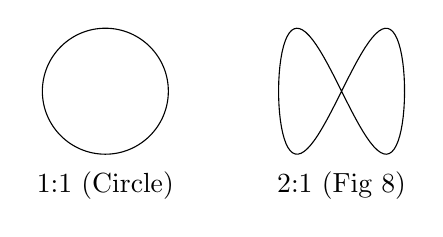
\begin{tikzpicture}
    % 1:1 Circle
    \draw (0,0) circle (0.8); \node at (0,-1.2) {1:1 (Circle)};
    % 2:1 Figure 8
    \draw [xshift=3cm, domain=0:360, samples=100] plot ({0.8*sin(\x)}, {0.8*sin(2*\x)}); \node at (3,-1.2) {2:1 (Fig 8)};
\end{tikzpicture}
\captionof{figure}{Lissajous Patterns}
\end{center}
\end{solutionbox}

\begin{mnemonicbox}
\mnemonic{XTYN: X-Tangents to Y-tangents gives the Number ratio}
\end{mnemonicbox}

\questionmarks{3(c)}{7}{Explain CRO with help of Block diagram.}

\begin{solutionbox}
\textbf{Cathode Ray Oscilloscope (CRO)} displays signal voltage vs time.

\textbf{Block Diagram}:
\begin{center}
\begin{tikzpicture}[node distance=1.5cm, auto]
    \node [gtu block] (VA) {Vert Amp};
    \node [gtu block, below=of VA] (DL) {Delay Line};
    \node [coordinate, left=of VA] (In) {};
    \node [gtu block, right=of DL] (CRT) {CRT};
    \node [gtu block, below=of DL] (Trig) {Trigger};
    \node [gtu block, right=of Trig] (TB) {Time Base};
    \node [gtu block, right=of TB] (HA) {Horiz Amp};
    \node [gtu block, below=of Trig] (PS) {Power Supply};
    
    \draw [gtu arrow] (In) -- node[above]{Input} (VA);
    \draw [gtu arrow] (VA) -- (DL);
    \draw [gtu arrow] (DL) -- (CRT);
    \draw [gtu arrow] (VA) |- (Trig);
    \draw [gtu arrow] (Trig) -- (TB);
    \draw [gtu arrow] (TB) -- (HA);
    \draw [gtu arrow] (HA) -| (CRT);
    \draw [gtu arrow] (PS) -| (CRT);
\end{tikzpicture}
\captionof{figure}{CRO Block Diagram}
\end{center}

\textbf{Key Blocks}:
\begin{itemize}
    \item \keyword{Vertical Amplifier}: Strengthens input signal.
    \item \keyword{Delay Line}: Delays vertical signal so horizontal sweep can start.
    \item \keyword{Time Base}: Generates sawtooth wave for horizontal deflection.
    \item \keyword{Trigger}: Synchronizes sweep with signal.
    \item \keyword{CRT}: Displays the electron beam trace.
\end{itemize}
\end{solutionbox}

\begin{mnemonicbox}
\mnemonic{VCTHP: Vertical input, Conditioned signal, Triggered sweep, Horizontal deflection, Phosphor display}
\end{mnemonicbox}

\questionmarks{3(a) OR}{3}{Explain different types of CRO probes.}

\begin{solutionbox}
\textbf{CRO Probes} connect the test circuit to the oscilloscope.

\begin{center}
\captionof{table}{Types of Probes}
\begin{tabulary}{\linewidth}{|L|L|}
\hline
\textbf{Type} & \textbf{Characteristics} \\ \hline
\textbf{Passive Probe} & Rugged, simple, 1:1 or 10:1 attenuation. High input impedance. \\ \hline
\textbf{Active Probe} & Built-in FET amplifier. Low capacitance, high bandwidth. Requires power. \\ \hline
\textbf{Current Probe} & Measures current via magnetic field (clip-on). No circuit breaking. \\ \hline
\textbf{Differential Probe} & Measures voltage difference between two points, rejecting common mode noise. \\ \hline
\end{tabulary}
\end{center}
\end{solutionbox}

\begin{mnemonicbox}
\mnemonic{PACD: Passive, Active, Current, Differential}
\end{mnemonicbox}

\questionmarks{3(b) OR}{4}{Draw internal structure of CRT. Explain in brief.}

\begin{solutionbox}
\textbf{CRT (Cathode Ray Tube)} is a vacuum tube that produces visual display.

\textbf{Structure Diagram}:
\begin{center}
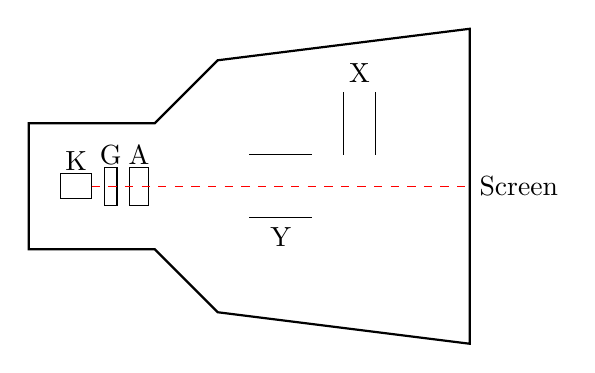
\begin{tikzpicture}[xscale=0.8, yscale=0.8]
    % Glass envelope
    \draw [thick] (0,1) -- (2,1) -- (3,2) -- (7,2.5) -- (7,-2.5) -- (3,-2) -- (2,-1) -- (0,-1) -- cycle;
    \node at (7,0) [right] {Screen};
    
    % Gun components
    \draw (0.5,-0.2) rectangle (1,0.2); \node at (0.75,0.4) {K}; % Cathode
    \draw (1.2,-0.3) rectangle (1.4,0.3); \node at (1.3,0.5) {G}; % Grid
    \draw (1.6,-0.3) rectangle (1.9,0.3); \node at (1.75,0.5) {A}; % Anodes
    
    % Deflection Plates
    \draw (3.5, 0.5) -- (4.5, 0.5); \draw (3.5, -0.5) -- (4.5, -0.5); \node at (4, -0.8) {Y};
    \draw (5, 0.5) -- (5, 1.5); \draw (5.5, 0.5) -- (5.5, 1.5); \node at (5.25, 1.8) {X};
    
    % Beam
    \draw [dashed, red] (1,0) -- (7,0);
\end{tikzpicture}
\captionof{figure}{CRT Construction}
\end{center}

\textbf{Parts}:
\begin{itemize}
    \item \keyword{Electron Gun}: K, G, A produce focused beam.
    \item \keyword{Deflection Plates}: Y-plates (Vertical) and X-plates (Horizontal) move the beam.
    \item \keyword{Screen}: Coated with phosphor, glows when hit by electrons.
\end{itemize}
\end{solutionbox}

\begin{mnemonicbox}
\mnemonic{GAFDS: Gun Aims, Focusing Directs, Screen shows}
\end{mnemonicbox}

\questionmarks{3(c) OR}{7}{Draw and explain block diagram of DSO in detail.}

\begin{solutionbox}
\textbf{Digital Storage Oscilloscope (DSO)} digitizes and stores waveforms.

\textbf{Block Diagram}:
\begin{center}
\begin{tikzpicture}[node distance=1.5cm, auto]
    \node [gtu block] (ADC) {ADC};
    \node [gtu block, left=of ADC] (Cond) {Signal Cond.};
    \node [coordinate, left=of Cond] (In) {};
    \node [gtu block, right=of ADC] (Mem) {Memory};
    \node [gtu block, right=of Mem] (Proc) {Processor};
    \node [gtu block, below=of Proc] (Disp) {Display};
    \node [gtu block, below=of ADC] (Cont) {Control/Clock};
    
    \draw [gtu arrow] (In) -- (Cond);
    \draw [gtu arrow] (Cond) -- (ADC);
    \draw [gtu arrow] (ADC) -- (Mem);
    \draw [gtu arrow] (Mem) -- (Proc);
    \draw [gtu arrow] (Proc) -- (Disp);
    \draw [gtu arrow] (Cont) -- (ADC);
    \draw [gtu arrow] (Cont) -- (Mem);
\end{tikzpicture}
\captionof{figure}{DSO Block Diagram}
\end{center}

\textbf{Working}:
\begin{enumerate}
    \item Input signal is conditioned (amplified/attenuated).
    \item \keyword{ADC} samples the signal and converts to binary data.
    \item Data is stored in \keyword{Digital Memory}.
    \item \keyword{Microprocessor} reads memory and reconstructs waveform for display.
\end{enumerate}
\end{solutionbox}

\begin{mnemonicbox}
\mnemonic{SAMPLE-D: Signal Acquisition, Memory Processing, Locking trigger, Display}
\end{mnemonicbox}

\questionmarks{4(a)}{3}{Give the comparison of NTC and PTC thermistor.}

\begin{solutionbox}
\begin{center}
\captionof{table}{NTC vs PTC Thermistor}
\begin{tabulary}{\linewidth}{|L|L|L|}
\hline
\textbf{Parameter} & \textbf{NTC (Negative Temp Coeff)} & \textbf{PTC (Positive Temp Coeff)} \\ \hline
Resistance Change & Decreases as Temp Increases & Increases as Temp Increases \\ \hline
Material & Semiconductor oxides (Mn, Ni) & Barium Titanate \\ \hline
Linearity & Non-linear (Exponential) & Non-linear (Sharp rise) \\ \hline
Application & Temp measurement, Compensation & Overcurrent protection, Heating \\ \hline
\end{tabulary}
\end{center}
\end{solutionbox}

\begin{mnemonicbox}
\mnemonic{IN-DP: Increase Negative, Decrease Positive}
\end{mnemonicbox}

\questionmarks{4(b)}{4}{Explain working principle and construction of Thermocouple.}

\begin{solutionbox}
\textbf{Thermocouple} measures temperature based on Seebeck Effect.

\textbf{Construction}: Two dissimilar metal wires joined at one end (Hot Junction). The other ends (Cold Junction) go to the meter.

\textbf{Diagram}:
\begin{center}
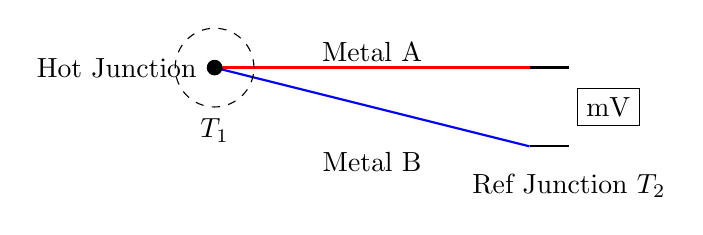
\begin{tikzpicture}
    \draw [thick, red] (0,0) -- (4,0); \node at (2, 0.2) {Metal A};
    \draw [thick, blue] (0,0) -- (4, -1); \node at (2, -1.2) {Metal B};
    
    \node [circle, fill, inner sep=2pt, label=left:Hot Junction] at (0,0) {};
    
    \draw [thick] (4,0) -- (4.5,0);
    \draw [thick] (4,-1) -- (4.5,-1);
    \node [draw] at (5, -0.5) {mV};
    
    \draw [dashed] (0,0) circle (0.5); \node at (0, -0.8) {$T_1$};
    \node at (4.5, -1.5) {Ref Junction $T_2$};
\end{tikzpicture}
\captionof{figure}{Thermocouple}
\end{center}

\textbf{Principle}: When two different metals are joined and junctions are at different temperatures ($T_1 \neq T_2$), an electromotive force (EMF) is generated. $E = k(T_1 - T_2)$.
\end{solutionbox}

\begin{mnemonicbox}
\mnemonic{STEM: Seebeck-effect Transforms temperature to EMF in Metals}
\end{mnemonicbox}

\questionmarks{4(c)}{7}{Explain Working of strain Gauge and Load cell. Give advantages and disadvantages of RTD.}

\begin{solutionbox}
\textbf{Strain Gauge}: Measures mechanical strain.
\begin{itemize}
    \item \keyword{Variable Resistance Transducer}.
    \item Construction: Fine wire grid on paper/backing.
    \item Working: Tension $\rightarrow$ Length $\uparrow$, Area $\downarrow$ $\rightarrow$ Resistance $\uparrow$.
    \item Gauge Factor $G.F. = \frac{\Delta R / R}{\Delta L / L}$.
\end{itemize}

\textbf{Load Cell}: Force transducer.
\begin{itemize}
    \item Uses strain gauges bonded to a metal element (column/beam).
    \item Force causes deformation, detected by strain gauges in Wheatstone bridge.
\end{itemize}

\textbf{RTD (Resistance Temperature Detector)}:
\begin{itemize}
    \item \textbf{Advantages}: High accuracy, stable, linear.
    \item \textbf{Disadvantages}: Self-heating, slower response than thermocouple, external power needed.
\end{itemize}
\end{solutionbox}

\begin{mnemonicbox}
\mnemonic{SPANNER: Strain Proportionally Alters Nominal Nominal Electrical Resistance}
\end{mnemonicbox}

\questionmarks{4(a) OR}{3}{Explain Humidity Sensor Hygrometer.}

\begin{solutionbox}
\textbf{Humidity Sensor (Hygrometer)} measures relative humidity (RH).

\textbf{Types}:
\begin{itemize}
    \item \keyword{Resistive}: Hygroscopic material absorbs moisture $\rightarrow$ Resistance decreases.
    \item \keyword{Capacitive}: Moisture absorption changes dielectric constant $\rightarrow$ Capacitance changes.
\end{itemize}

\textbf{Block Diagram}:
\begin{center}
\begin{tikzpicture}[node distance=1.5cm, auto]
    \node [gtu block] (Sens) {Sensing Element};
    \node [gtu block, right=of Sens] (Cond) {Signal Cond.};
    \node [gtu block, right=of Cond] (Disp) {Display};
    \node [left=of Sens] (Air) {Moist Air};
    
    \draw [gtu arrow] (Air) -- (Sens);
    \draw [gtu arrow] (Sens) -- (Cond);
    \draw [gtu arrow] (Cond) -- (Disp);
\end{tikzpicture}
\captionof{figure}{Humidity Sensor}
\end{center}
\end{solutionbox}

\begin{mnemonicbox}
\mnemonic{CRT-H: Capacitance/Resistance/Thermal changes with Humidity}
\end{mnemonicbox}

\questionmarks{4(b) OR}{4}{Draw and explain Piezoelectric transducer.}

\begin{solutionbox}
\textbf{Piezoelectric Transducer} converts pressure/acceleration to voltage.

\textbf{Diagram}:
\begin{center}
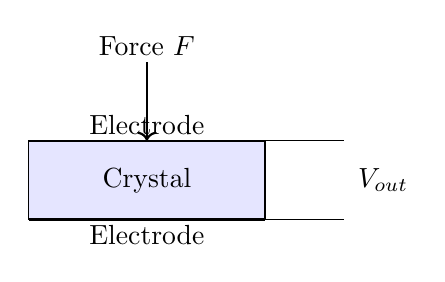
\begin{tikzpicture}
    \draw [fill=blue!10] (0,0) rectangle (3,1); \node at (1.5,0.5) {Crystal};
    \draw [thick] (0,1) -- (3,1); \node at (1.5,1.2) {Electrode};
    \draw [thick] (0,0) -- (3,0); \node at (1.5,-0.2) {Electrode};
    
    \draw [->, thick] (1.5, 2) -- (1.5, 1); \node at (1.5, 2.2) {Force $F$};
    \draw (3,1) -- (4,1); \draw (3,0) -- (4,0);
    \node at (4.5, 0.5) {$V_{out}$};
\end{tikzpicture}
\captionof{figure}{Piezoelectric Crystal}
\end{center}

\textbf{Working}:
\begin{itemize}
    \item Based on \keyword{Piezoelectric Effect}.
    \item When pressure is applied to crystal (Quartz, Rochelle Salt, PZT), charges accumulate on faces.
    \item $V = Q/C = d \cdot F / C$.
    \item \textbf{Active Transducer} (Self-generating).
\end{itemize}
\end{solutionbox}

\begin{mnemonicbox}
\mnemonic{PEMS: Pressure Ensures Measurable Signal}
\end{mnemonicbox}

\questionmarks{4(c) OR}{7}{Give the classification of transducers in detail.}

\begin{solutionbox}
\textbf{Transducer Classification}:

\begin{enumerate}
    \item \textbf{Based on Transduction Principle}:
    \begin{itemize}
        \item Resistive (Potentiometer, Strain Gauge)
        \item Capacitive (Var distance, dielectric)
        \item Inductive (LVDT)
        \item Piezoelectric
        \item Photovoltaic/Photoconductive
    \end{itemize}
    \item \textbf{Active vs Passive}:
    \begin{itemize}
        \item \keyword{Active}: Generates own voltage (Thermocouple, Piezo).
        \item \keyword{Passive}: Needs external power (RTD, Strain Gauge, LVDT).
    \end{itemize}
    \item \textbf{Primary vs Secondary}:
    \begin{itemize}
        \item \keyword{Primary}: Detects physical phenomenon (Bourdon Tube).
        \item \keyword{Secondary}: Converts primary output to electrical (LVDT on Bourdon).
    \end{itemize}
    \item \textbf{Analog vs Digital}:
    \begin{itemize}
        \item Analog: Continuous output.
        \item Digital: Pulse/Binary output (Encoders).
    \end{itemize}
\end{enumerate}
\end{solutionbox}

\begin{mnemonicbox}
\mnemonic{APAD RICE: Active/Passive, Analog/Digital with Resistive, Inductive, Capacitive, Electromagnetic}
\end{mnemonicbox}

\questionmarks{5(a)}{3}{Write short note on various Capacitive transducer.}

\begin{solutionbox}
\textbf{Capacitive Transducers} work on $C = \frac{\epsilon A}{d}$.

\textbf{Types}:
\begin{enumerate}
    \item \textbf{Variable Separation ($d$)}: Moving plate changes distance. Used for displacement, pressure.
    \item \textbf{Variable Area ($A$)}: Moving plate overlaps fixed plate distinctively. Used for large displacement.
    \item \textbf{Variable Dielectric ($\epsilon$)}: Dielectric material moves between plates. Used for liquid level.
\end{enumerate}
\end{solutionbox}

\begin{mnemonicbox}
\mnemonic{PALD: Parameter Alters the Leading Dielectric}
\end{mnemonicbox}

\questionmarks{5(b)}{4}{Explain LVDT Transducer.}

\begin{solutionbox}
\textbf{LVDT (Linear Variable Differential Transformer)} is an inductive transducer for linear displacement.

\textbf{Construction Diagram}:
\begin{center}
\begin{circuitikz}[american, scale=0.8]
    % Core
    \draw [fill=gray!30] (1,3) rectangle (3,5);
    \node at (2,4) {Core};
    \draw [->, thick] (2,5.2) -- (2,5.8) node[above] {Disp.};

    % Primary
    \draw (0,3.5) to[L, l=$P$] (0,4.5);
    \draw (-1,3.5) to[sV, l=$V_{in}$] (-1,4.5);
    \draw (-1,3.5) -- (0,3.5); \draw (-1,4.5) -- (0,4.5);

    % Secondaries
    \draw (4,5) to[L, l=$S_1$] (4,6);
    \draw (4,2) to[L, l=$S_2$] (4,3);
    
    % Series Opp
    \draw (4,3) -- (4,5);
    \draw (4,6) -- (5,6) node[right] {+};
    \draw (4,2) -- (5,2) node[right] {-};
    \node at (5.5, 4) {$V_{out}$};
\end{circuitikz}
\captionof{figure}{LVDT Construction}
\end{center}

\textbf{Working}:
\begin{itemize}
    \item Primary powered by AC.
    \item Voltage induced in secondaries depends on core position.
    \item Secondaries connected in \keyword{Series Opposition}: $V_{out} = V_{s1} - V_{s2}$.
    \item At center (Null): $V_{out} = 0$.
\end{itemize}
\end{solutionbox}

\begin{mnemonicbox}
\mnemonic{MDVN: Movement Determines Voltage from Null}
\end{mnemonicbox}

\questionmarks{5(c)}{7}{Draw and explain Harmonics Distortion Analyzer.}

\begin{solutionbox}
\textbf{Harmonic Distortion Analyzer} measures Total Harmonic Distortion (THD).

\textbf{Block Diagram}:
\begin{center}
\begin{tikzpicture}[node distance=1.5cm, auto]
    \node [gtu block] (Imp) {Impedance Conv.};
    \node [gtu block, left=of Imp] (In) {Input};
    \node [gtu block, right=of Imp] (Notch) {Notch Filter};
    \node [gtu block, right=of Notch] (Amp) {Amplifier};
    \node [gtu block, right=of Amp] (Meter) {Meter};
    
    \draw [gtu arrow] (In) -- (Imp);
    \draw [gtu arrow] (Imp) -- (Notch);
    \draw [gtu arrow] (Notch) -- (Amp);
    \draw [gtu arrow] (Amp) -- (Meter);
    
    % Switch bypass
    \draw [dashed] (Imp) -- ++(0,-1) -| (Amp); \node at (1.5, -1.2) {100\% Set (Bypass Filter)};
\end{tikzpicture}
\captionof{figure}{Fundamental Suppression Analyzer}
\end{center}

\textbf{Working}:
\begin{enumerate}
    \item \keyword{Set Level}: Filter bypassed. Meter reads total signal (Fundamental + Harmonics). Adjust gain to mark 100\%.
    \item \keyword{Measure}: Filter inserted. Fundamental frequency removed. Meter measures remaining harmonics.
    \item $THD = \frac{\sqrt{\sum V_n^2}}{V_1}$.
\end{enumerate}
\end{solutionbox}

\begin{mnemonicbox}
\mnemonic{FAIR-D: Filter And Isolate Residuals for Distortion}
\end{mnemonicbox}

\questionmarks{5(a) OR}{3}{Explain the working principle of Proximity sensors.}

\begin{solutionbox}
\textbf{Proximity Sensors} detect presence of objects without contact.

\textbf{Types}:
\begin{itemize}
    \item \keyword{Inductive}: Detects metal objects via eddy currents.
    \item \keyword{Capacitive}: Detects any object by dielectric change.
    \item \keyword{Optical}: Detects via light beam interruption/reflection.
\end{itemize}

\textbf{Working}: An electromagnetic or electrostatic field is emitted. Object entering the field changes field properties (damping oscillation or changing capacitance), triggering switching circuit.
\end{solutionbox}

\begin{mnemonicbox}
\mnemonic{CUPS: Capacitive, Ultrasonic, Photoelectric, Sense}
\end{mnemonicbox}

\questionmarks{5(b) OR}{4}{Explain absolute and incremental type of Optical encoder.}

\begin{solutionbox}
\textbf{Optical Encoder} measures angular position/speed.

\textbf{Absolute Encoder}:
\begin{itemize}
    \item Disc has multiple tracks with unique binary code for each angle.
    \item Outputs absolute position immediately.
    \item Doesn't lose position on power loss.
\end{itemize}

\textbf{Incremental Encoder}:
\begin{itemize}
    \item Disc has slots on periphery.
    \item Outputs pulses as it rotates.
    \item Measures speed and relative change.
    \item Loses position on power loss.
\end{itemize}

\textbf{Diagram}:
\begin{center}
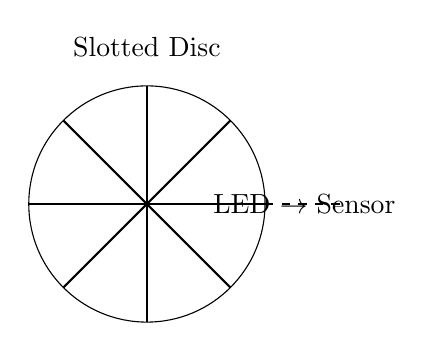
\begin{tikzpicture}
    % Disc
    \draw (0,0) circle (1.5);
    \foreach \x in {0, 45, ..., 360} \draw [thick] (0,0) -- (\x:1.5);
    \node at (0,2) {Slotted Disc};
    
    % LED/Sensor
    \node at (2,0) {LED $\rightarrow$ Sensor};
    \draw [dashed] (1.5, 0) -- (2.5, 0);
\end{tikzpicture}
\captionof{figure}{Basic Encoder Principle}
\end{center}
\end{solutionbox}

\begin{mnemonicbox}
\mnemonic{APIR-CD: Absolute Provides Immediate Reading, Counter Determines incremental}
\end{mnemonicbox}

\questionmarks{5(c) OR}{7}{Write short note on Digital IC Tester.}

\begin{solutionbox}
\textbf{Digital IC Tester} checks functionality of logic gates, Flip-flops, etc.

\textbf{Block Diagram}:
\begin{center}
\begin{tikzpicture}[node distance=1.5cm, auto]
    \node [gtu block] (CPU) {CPU};
    \node [gtu block, below=of CPU] (Mem) {Pattern ROM};
    \node [gtu block, right=of CPU] (Socket) {ZIF Socket};
    \node [gtu block, right=of Socket] (Comp) {Comparator};
    \node [gtu block, left=of CPU] (Disp) {Display/Keypad};
    
    \draw [gtu arrow] (CPU) -- (Socket);
    \draw [gtu arrow] (Mem) -- (CPU);
    \draw [gtu arrow] (Socket) -- (Comp);
    \draw [gtu arrow] (Comp) -- node[above]{Pass/Fail} (CPU);
    \draw [gtu arrow] (Disp) -- (CPU);
\end{tikzpicture}
\captionof{figure}{IC Tester}
\end{center}

\textbf{Operation}:
\begin{enumerate}
    \item User enters IC number (e.g., 7400).
    \item CPU fetches truth table from ROM.
    \item CPU applies inputs to IC Pins via ZIF socket.
    \item Comparator compares actual outputs with expected outputs.
    \item If all match $\rightarrow$ PASS. Else $\rightarrow$ FAIL.
\end{enumerate}
\end{solutionbox}

\begin{mnemonicbox}
\mnemonic{GATES: Generate And Test Every Signal}
\end{mnemonicbox}

\end{document}
